% --- Slide 1: Self-Occlusion & The Need for Inpainting ---
\begin{frame}{Self-Occlusion \& Inpainting}
    \begin{columns}[c]
        \begin{column}{0.48\textwidth}
            \begin{block}{The Problem}
                \small
                \begin{itemize}
                    \item Turning head or opening mouth reveals parts not visible in source $S$ (teeth, tongue, cheeks).
                    \item Pure warping has no pixels to sample from $\to$ stretches or leaves black holes.
                \end{itemize}
            \end{block}

            \begin{block}{The Fix}
                \small
                \begin{itemize}
                    \item \textbf{Occlusion Mask ($O$):} Flags missing pixels ($O \approx 0$).
                    \item \textbf{Inpainting:} Generator fills missing pixels using facial patterns learned during training.
                \end{itemize}
            \end{block}
        \end{column}

        \begin{column}{0.50\textwidth}
            \centering
            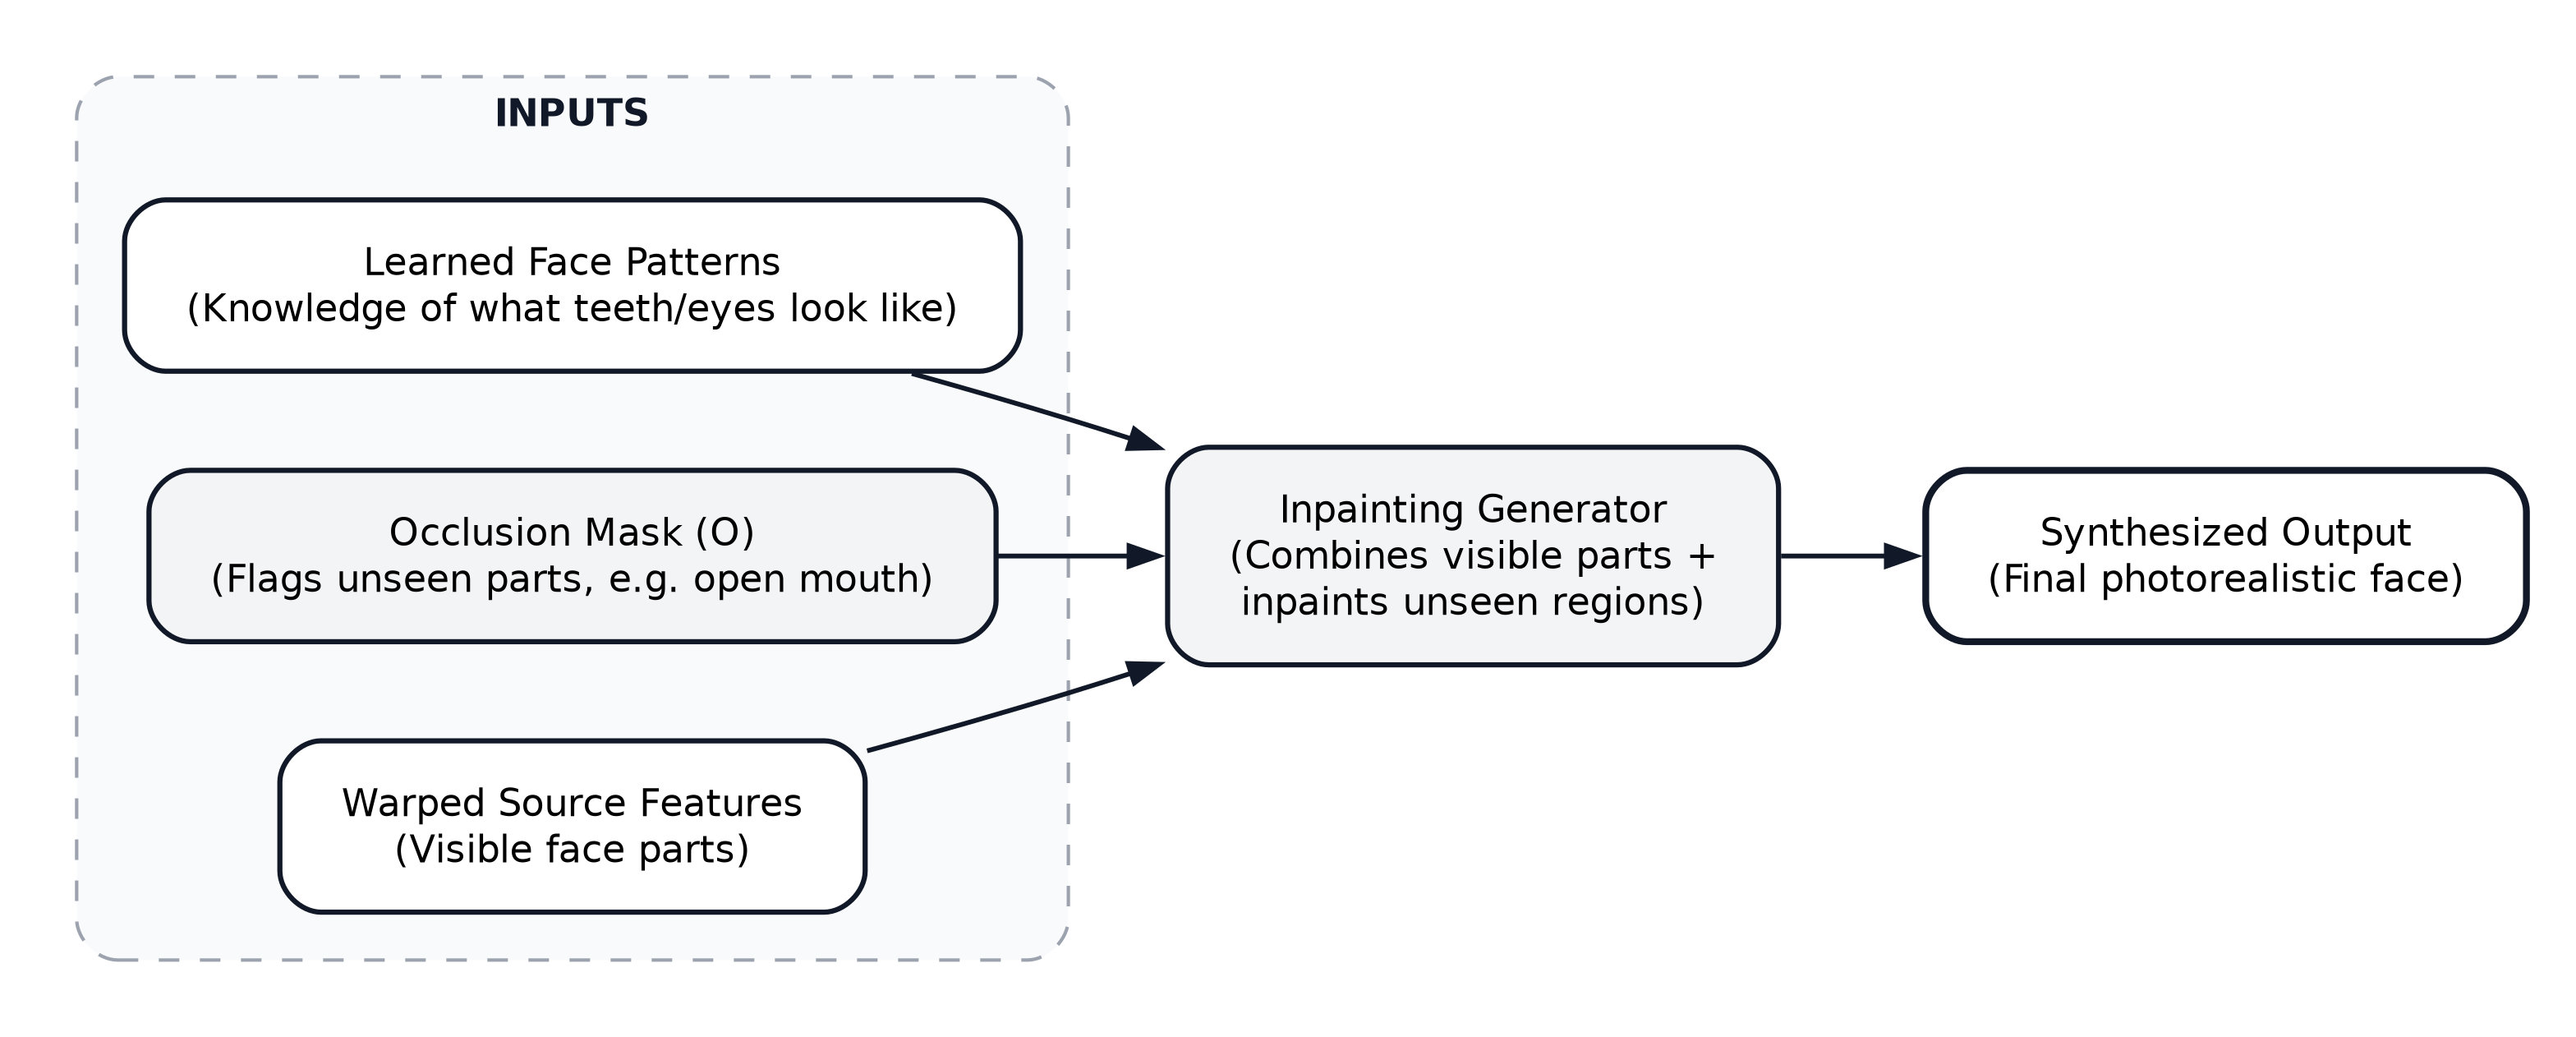
\includegraphics[width=\linewidth, height=4.2cm, keepaspectratio]{diagram_occlusion_inpainting.png}
        \end{column}
    \end{columns}
\end{frame}

% --- Slide 2: Visual Proof of Pipeline Execution (Intermediate Stages) ---
\begin{frame}{Pipeline Verification: Intermediate Stages}
    \begin{center}
        \small \textbf{5 Intermediate Stages Extracted During Local Inference}
    \end{center}
    
    \vspace{-0.1cm}
    \begin{center}
        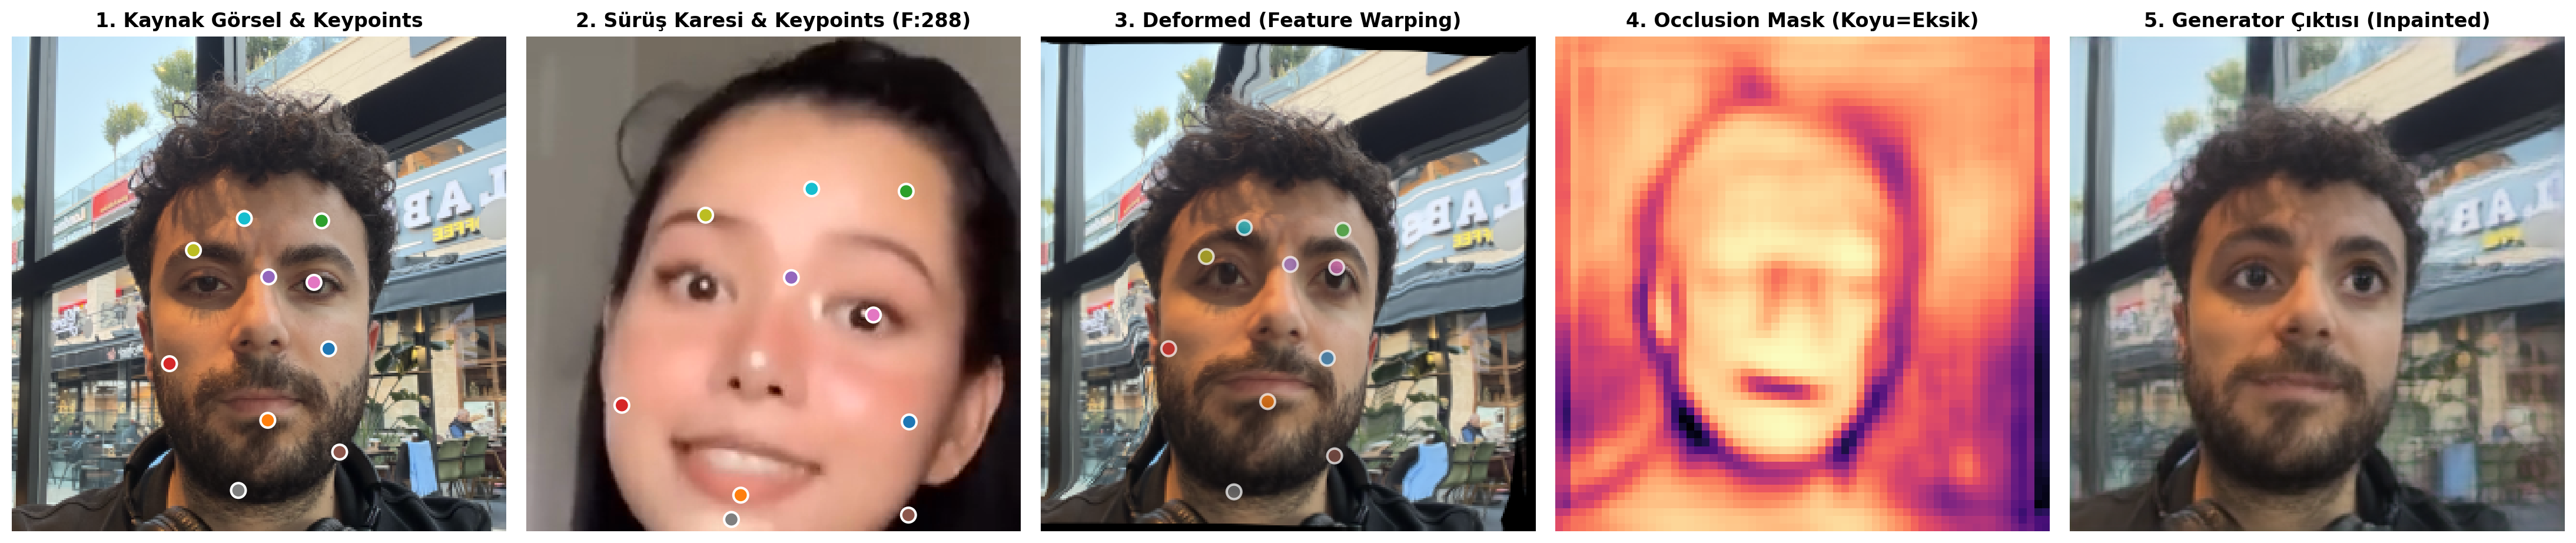
\includegraphics[width=0.96\linewidth, height=3.5cm, keepaspectratio]{ara_asamalar_gorsellestirme.png}
    \end{center}
    \vspace{-0.1cm}
    
    \begin{columns}[T]
        \begin{column}{0.19\textwidth}
            \centering \scriptsize \textbf{1. Source Points}\\
            $S$ reference keypoints
        \end{column}
        \begin{column}{0.19\textwidth}
            \centering \scriptsize \textbf{2. Driving Points}\\
            $D$ tracking points
        \end{column}
        \begin{column}{0.19\textwidth}
            \centering \scriptsize \textbf{3. Warped Frame}\\
            Flow-deformed source
        \end{column}
        \begin{column}{0.19\textwidth}
            \centering \scriptsize \textbf{4. Occlusion Mask}\\
            Dark = missing regions
        \end{column}
        \begin{column}{0.19\textwidth}
            \centering \scriptsize \textbf{5. Inpainted Result}\\
            Synthesized output
        \end{column}
    \end{columns}
\end{frame}
